% \newpage

\subsubsection*{Т22}

Вычислим хаусдорфову размерность для обобщения кривой Коха, с углом между линиями $\theta$. Примеры построения кривой на разных шагах приведены на рисунке \ref{fig:koch}.
\begin{figure}[h]
    \centering
    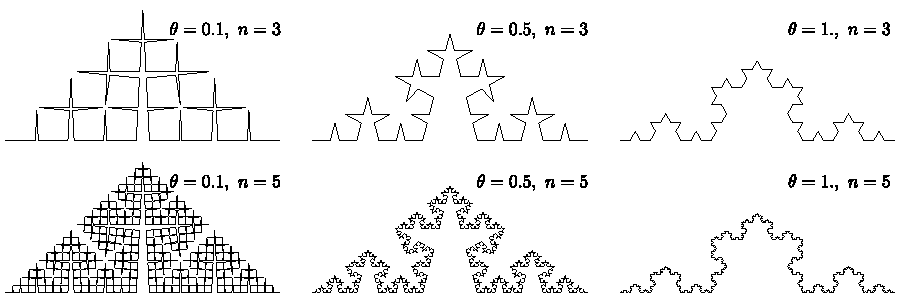
\includegraphics[width=0.7\textwidth]{figures/koch_line.pdf}
    \caption{Кривая из Т22 при разных параметрах $\theta, n$}
    \label{fig:koch}
\end{figure}
Для начала поймём, что на $n$-ном шаге всего будет $N = 4^n$ звеньев, длины $\rho$ каждый. Понятно, что
\begin{equation*}
    \sin \frac{\theta}{2} = \left(\frac{\rho_n - 2 \rho_{n+1}}{2}\right) \bigg/ \rho = \frac{\rho_n}{2 \rho_{n+1}} - 1,
    \hspace{0.5cm} \Rightarrow \hspace{0.5cm}
    \rho_n = \frac{\rho_0}{\left[
        2 +2 \sin(\theta/2)
    \right]^n}.
\end{equation*}
Длину кривой мы можем найти, как $N(\varepsilon)$ отрезков длины $\varepsilon = \rho$, тогда искомая размерность кривой
\begin{equation*}
    \textnormal{dim}(\theta) = \lim_{n \to \infty} \frac{
    \ln N(\varepsilon)
    }{
    \ln(1/\varepsilon)
    } = \lim_{n \to \infty} 
    \frac{\ln 4^n}{\ln\left[2(1+\sin \theta/2)\right]^n} = \frac{\ln 4}{\ln 2 + \ln \left[1+\sin \frac{\theta}{2}\right]},
\end{equation*}
что любопытно рассмотреть на некоторых частных случаях. 

В частности, что также видно из построения, при $\theta = 0$ кривая превратиться в некоторое покрытие плоскости умельчающейся сеткой, и $\textnormal{dim}(\theta=0) = 2$.
При $\theta = \pi/3$ мы придём к кривой Коха, с размерностью $\textnormal{dim}(\theta= \pi/3) = \ln 4/ \ln 3 \approx 1.26$, рисунок которой приведен посередине \eqref{fig:koch}. 
Наконец, при $\theta = \pi$ мы после каждой итерации будем получать прямую, и $\textnormal{dim}(\theta= \pi) = 1$. 

В случае, если мы будем говорить о размерности фигуры под рассматриваемой кривой, то обнаружим, что площадь на $n$-ной итерации может быть найдена, как
\begin{equation*}
    S_n = \frac{1}{2} \rho_0^2 \sin \theta \left[
        \frac{1}{4^2} + \frac{1}{4^3} + \ldots + \frac{1}{4^{n}}
    \right],
    \hspace{10 mm} 
    \lim_{n \to \infty} S_n = \frac{1}{24} \rho_0^2 \sin \theta,
\end{equation*}
таким образом нас интересует размерность плоской фигуры конечной площади, $N(\varepsilon) \sim \varepsilon^{-2}$ $\Rightarrow$ $\textnormal{dim} = 2$.